\documentclass[conference]{IEEEtran}

\usepackage[utf8]{inputenc}
\usepackage[T1]{fontenc}
\usepackage[english]{babel}
\usepackage{graphicx}
\usepackage{amsmath}
\usepackage{array}
\usepackage{booktabs}
\usepackage{url}
\usepackage{tikz}
\usetikzlibrary{shapes.geometric, arrows.meta, positioning, fit}
\hyphenation{em-bo-di-ment re-trieval}

\begin{document}

\title{Does Embodiment Help? Evaluating the Effect of a Corporeal Virtual
Agent on Trust and Interaction Naturalness in a RAG-Based Document
Consultation System}

\author{\authorblockN{Marco Antonio Jim\'{e}nez Guti\'{e}rrez}
\authorblockA{School of Computer Science and Informatics (ECCI)\\
University of Costa Rica\\
San Jos\'{e}, Costa Rica\\
marjimgu@gmail.com}}

\maketitle

\begin{abstract}
Document consultation systems based on Retrieval-Augmented Generation (RAG)
typically present answers in plain text, which may constrain the naturalness
and trust of the interaction. This paper presents Ariel, a web-native
corporeal virtual agent (CVA) implemented with Three.js and @pixiv/three-vrm
that acts as the front end of a RAG system for consulting document files in a
document-management platform. Ariel communicates generated answers through
synthesized speech and a 3D avatar with idle, listening and speaking
animations, latency cues, and emotional expressions controlled by a large language model
(LLM). We report
a between-subjects expert pilot ($N=8$) comparing the CVA (Condition~A)
against an equivalent text-only interface (Condition~B) that shares an
identical RAG and LLM back end, isolating the effect of embodiment. We measured
perceived trust (Trust in Automation, TiA), interaction naturalness (Godspeed),
usability (System Usability Scale, SUS) and factual retention. The CVA raised
perceived trust (TiA trust $4.83$ vs.\ $3.58$) but, as implemented, was rated
\emph{lower} on anthropomorphism ($1.60$ vs.\ $2.50$), animacy and likeability,
while usability (SUS $73.8$ vs.\ $72.5$) and retention ($2.25$ vs.\ $2.50$ of
$3$) were equivalent. Qualitative closing interviews attribute the naturalness
penalty to synthetic voice and simulated lip~sync rather than to embodiment
itself. We conclude that the bottleneck is multimodal fidelity, not the mere
presence of a body.
\end{abstract}

\IEEEoverridecommandlockouts
\begin{keywords}
Corporeal virtual agents, embodiment, RAG, perceived trust, HCI, VRM,
document consultation.
\end{keywords}

\IEEEpeerreviewmaketitle


% =====================================================================
\section{Introduction}
The management of document databases, particularly those organized through
archival techniques, requires consulting files that group multiple related
documents. Retrieval-Augmented Generation (RAG) connects such collections with
large language models (LLMs), enabling contextualized answers grounded in the
real content of the file \cite{fan2024,roy2024,haque2025}. However, most RAG
implementations present answers as plain text, much like a traditional chat
interface.

Although functional, this presentation mode can feel limited when the goal is a
consultation experience perceived as natural, close and trustworthy.
Human--computer interaction (HCI) studies suggest that the presence of a
corporeal virtual agent (CVA) can positively influence perceived trust,
interaction naturalness and answer comprehension \cite{wang2019,chang2022,
yang2025ar}. Yet specific evidence on CVAs applied to document RAG systems is
scarce, and it is not obvious that adding a body is beneficial in a task whose
value lies in factual precision.

This work investigates whether presenting RAG answers through a corporeal
virtual agent---with synthesized voice, animations and emotional
expressions---produces measurable differences in perceived trust and
interaction naturalness compared to an equivalent text interface. We present
Ariel, a CVA integrated in the RAG platform, and a comparative
evaluation protocol designed to answer the following research questions:

\begin{itemize}
\item \textbf{RQ1:} What effect does using a CVA as the front end of a RAG
system have on \emph{perceived trust} in the generated answers, compared with a
text-based document consultation interface?
\item \textbf{RQ2:} What effect does the CVA have on the \emph{perceived
naturalness} of the interaction and on comprehension of answers in document
consultation tasks, compared with a chat-style text interface?
\item \textbf{RQ3:} What effect does the CVA have on \emph{perceived usability}
and on \emph{information retention}, compared with a text interface?
\end{itemize}

Our contribution is threefold: (i) the design and implementation of Ariel as a
web-native CVA built with Three.js and the Virtual Reality Model (VRM) avatar
format, over a RAG back end; (ii) a controlled
between-subjects protocol that isolates embodiment; and (iii) empirical
evidence---quantitative and qualitative---showing a dissociation between trust
(improved by embodiment) and naturalness (degraded by low multimodal fidelity).
Section~\ref{sec:related} reviews related work; Section~\ref{sec:system}
describes Ariel; Section~\ref{sec:method} the study design;
Section~\ref{sec:results} the results; Section~\ref{sec:discussion} the
discussion; and Section~\ref{sec:conclusion} the conclusions.


% =====================================================================
\section{Related Work}
\label{sec:related}

\textbf{Retrieval-Augmented Generation.}
RAG systems overcome a central limitation of LLMs: their dependence on static,
internal knowledge. By integrating retrieval from external sources, RAG improves
relevance, currency and grounding of answers \cite{fan2024,roy2024,haque2025,
ahn2022}. A key finding is that the agent must be connected to a verifiable
document memory that reduces hallucinations and improves traceability
\cite{fan2024,roy2024}; knowledge-grounded conversation further requires local
context to stay coherent over long dialogues \cite{ahn2022}. PersonaRAG shows
that RAG improves when it incorporates user-centric agents that adapt retrieval
and generation to needs in real time \cite{zerhoudi2024}, a principle directly
applicable to Ariel \cite{more2025,schmitt2022}. Studies of user behavior with
generative information-retrieval systems highlight how users formulate and
verify queries \cite{liang2025}, while knowledge-adaptive generative agents
extend RAG toward up-to-date simulations \cite{shimadzu2025}.

\textbf{Corporeal virtual agents and interaction.}
Studies in augmented and virtual reality show that an agent's visual presence
can influence perceived intelligence, trust, closeness, usefulness and social
presence \cite{wang2019,chang2022,yang2025ar,zhu2024,koleva2024}. However, the
body must be designed with care: an agent that is overly anthropomorphic,
unnatural or poorly synchronized can produce discomfort or loss of trust---the
Uncanny Valley effect \cite{mori2012,wang2019}. Foundational work on embodied
conversational agents establishes that combining natural language with
non-verbal cues is fundamental to interactions perceived as natural
\cite{alalyani2023}, while research on relational trust shows that conversational
agents designed as explanatory, orienting interfaces favor perceived trust
\cite{schmitt2022}. Longitudinal studies of companion virtual agents further
show that engagement and user attitudes evolve over repeated sessions
\cite{calvo2025}.

\textbf{Latency, multimodality and lip~sync.}
Conversational naturalness depends on turn management, visual feedback and
latency. Pauses, facial expressions and waiting cues mitigate the negative
perception of latency in LLM-powered agents \cite{jolibois2025,elfleet2024};
allowing verbal interruptions improves perceived efficiency \cite{egelhofer2025}.
In browser speech-synthesis systems, lip~sync quality has been shown to affect
perceived naturalness and presence \cite{chang2022,elfleet2024}.

\textbf{Evaluation of CVAs.}
The LLM~+~RAG~+~multimodal-agent combination has outperformed purely textual,
scripted variants in task success and perceived naturalness, especially in
high-impact domains such as health, education and institutional services
\cite{yang2025health}. The most common instruments to evaluate CVAs are the
Godspeed Questionnaire \cite{bartneck2009}, the Trust in Automation scale (TiA)
\cite{jian2000} and the System Usability Scale (SUS) \cite{brooke1996},
combined with information-retention tasks to measure effective comprehension.


% =====================================================================
\section{System Design: Ariel}
\label{sec:system}

Ariel is a CVA integrated in a document-file management platform.
It acts as a consultation interface over the documents of the active file,
retrieving relevant information via RAG and communicating it through a 3D avatar
with synthesized voice. The system has three components: avatar rendering
(front end), the RAG pipeline (back end) and browser speech synthesis
(Fig.~\ref{fig:arch}); Fig.~\ref{fig:screenshot} shows the CVA condition in
operation.

\textbf{Front end.}
The avatar is rendered with \textbf{Three.js} and \textbf{@pixiv/three-vrm},
loading VRM avatars (a glTF-based humanoid-avatar format) directly in the
browser, with no external game engine; this removes the need for a Unity build
and improves reproducibility. The
\texttt{AvatarController} manages dynamic VRM loading with runtime model
swapping, a natural rest pose (arms lowered, head toward camera) applied from
the default T-pose, and procedural idle animations (sinusoidal breathing,
random blinking every 2--6\,s, gentle head sway). Because the Web Speech API does
not expose the audio stream, \emph{simulated} lip~sync is used: the
\texttt{onstart}, \texttt{onboundary} and \texttt{onend} events of
\texttt{SpeechSynthesisUtterance} drive the \texttt{Aa}/\texttt{Oh} blend shapes
during speech. The LLM can invoke emotional expressions (happy, sad, neutral,
surprised, relaxed, angry) mapped to VRM expressions with smooth interpolation.

\textbf{Back end.}
A secure intermediary (Node/Express locally, deployed as Firebase Cloud
Functions in production) processes each query in three stages:
(1)~\emph{retrieval} via semantic search over the active file's vector store;
(2)~\emph{generation}, integrating retrieved fragments as context for the LLM
(OpenAI GPT-4.1-nano) together with behavior instructions; and (3)~\emph{response},
returning text plus an emotion-action metadatum that the controller interprets.
\begin{figure}[t]
    \centering
    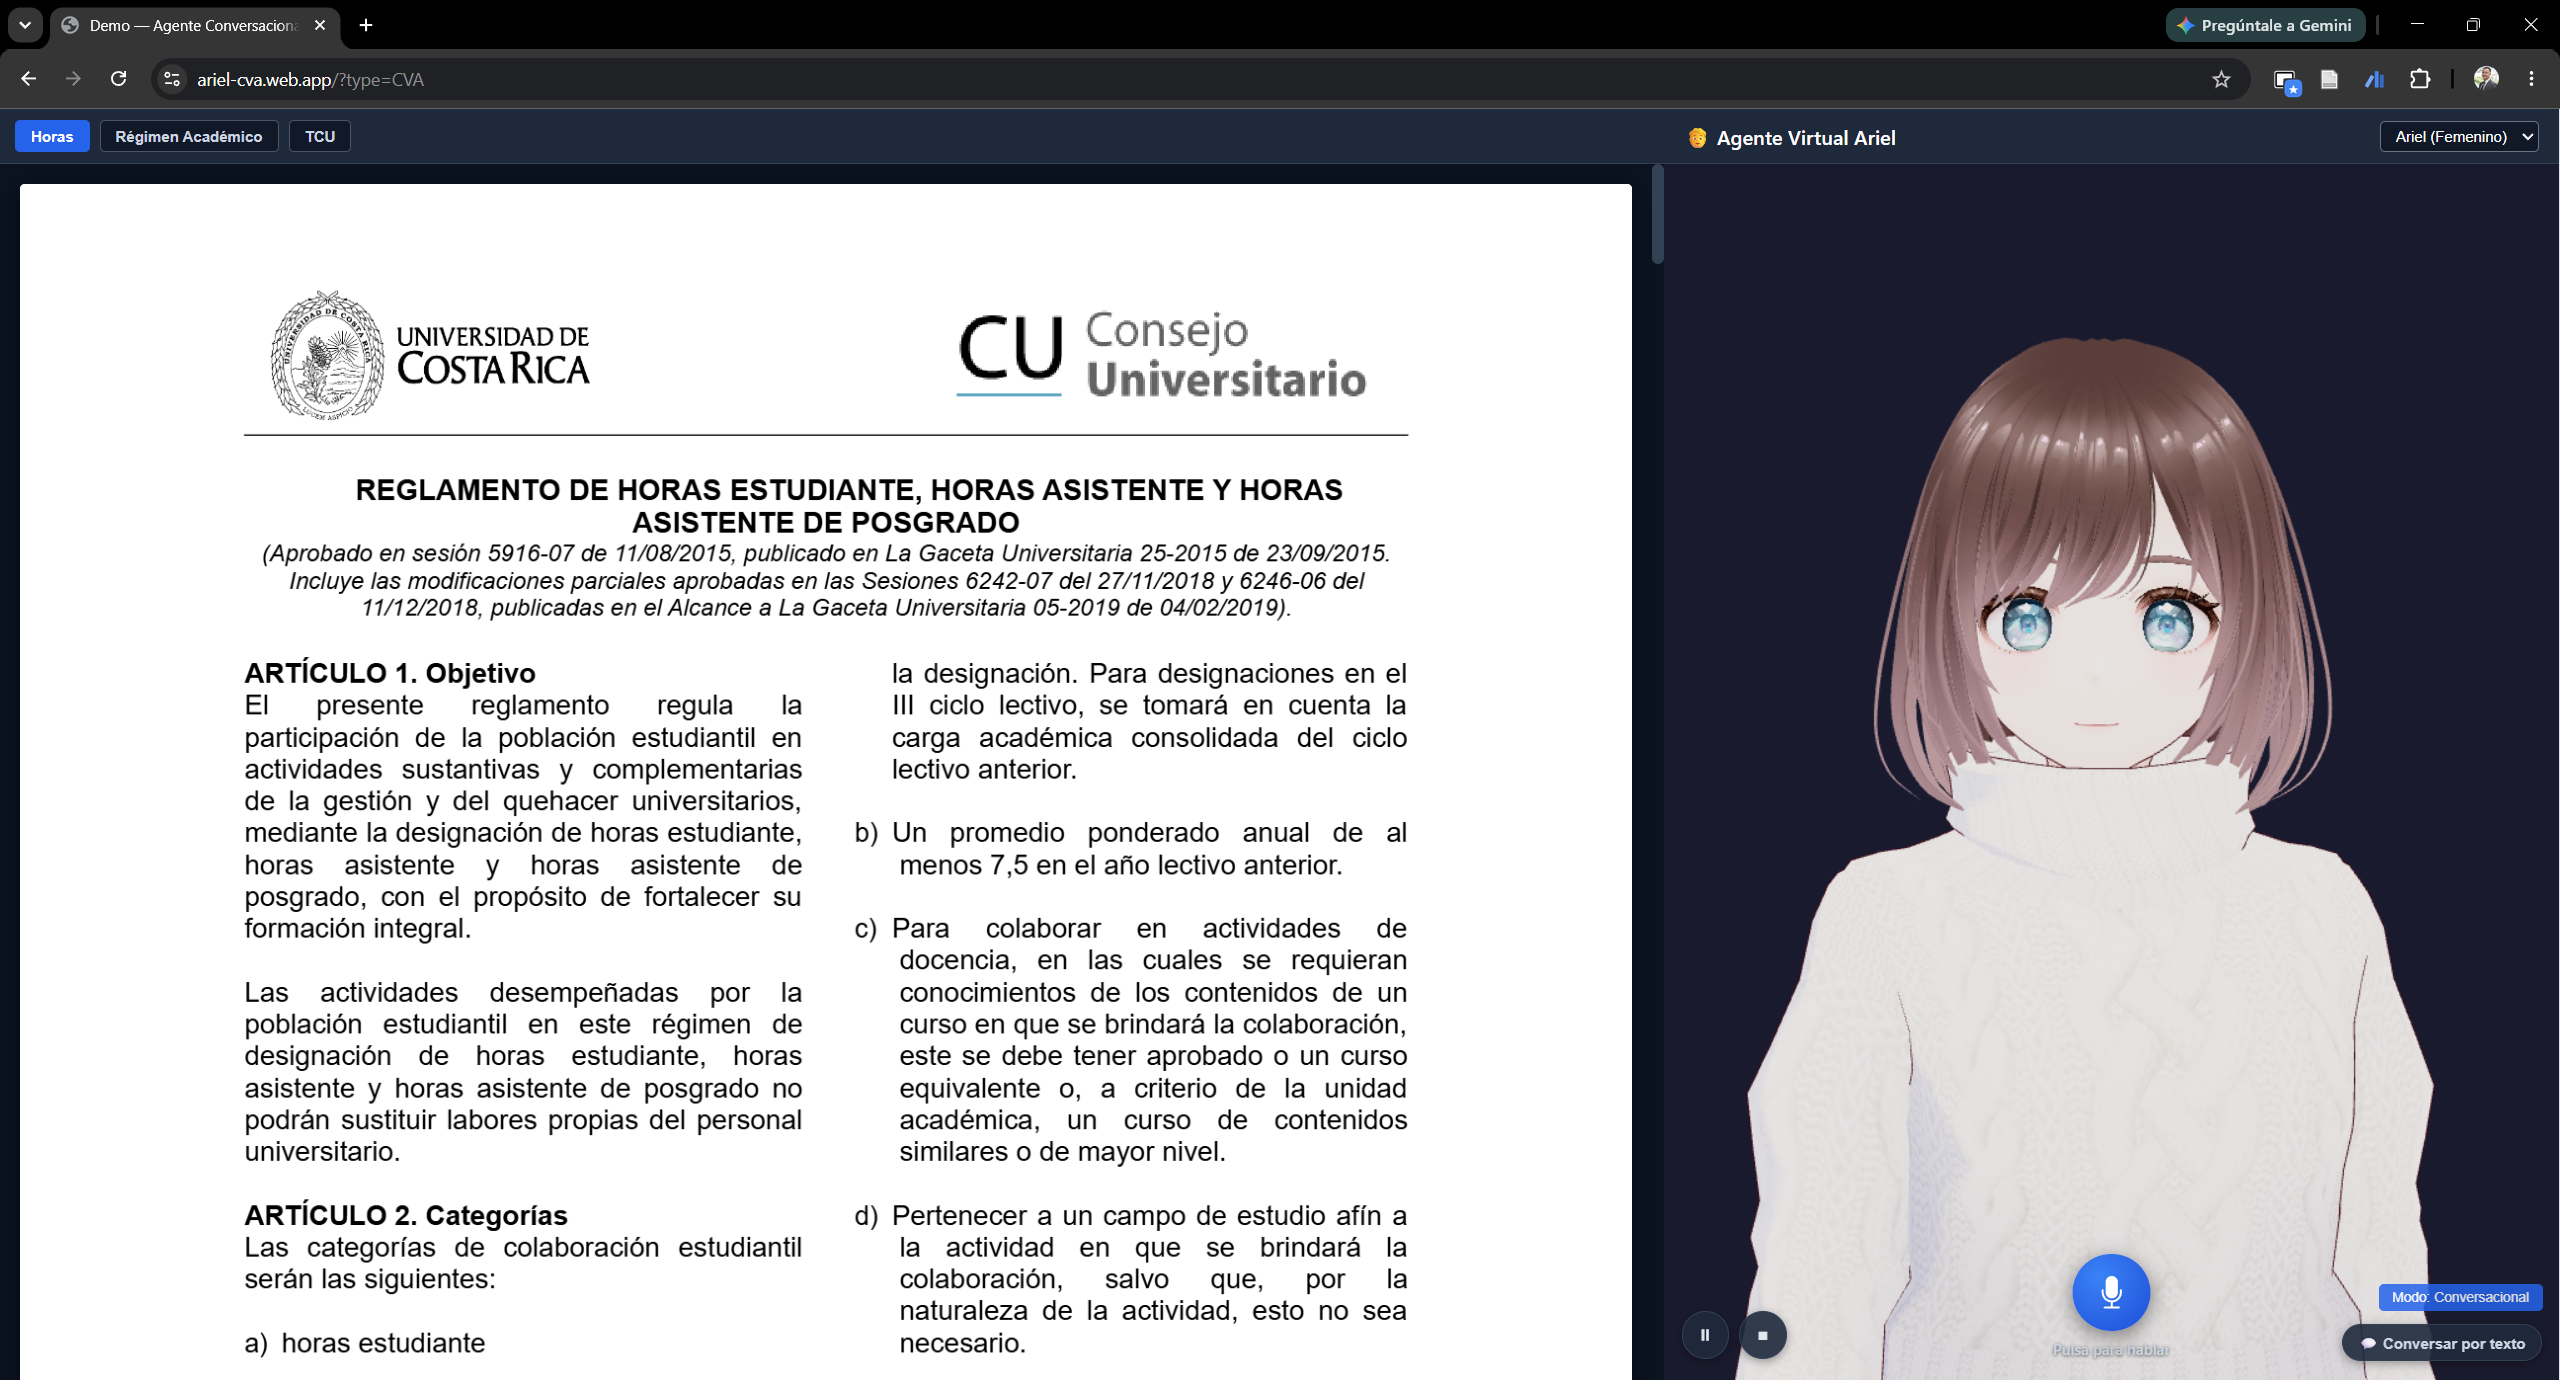
\includegraphics[width=\linewidth]{ariel.png}
    \caption{The CVA condition (Condition~A) in operation: the 3D avatar (right)
    is rendered beside the document viewer showing the active file---a University
    of Costa Rica regulation (left).}
    \label{fig:screenshot}
\end{figure}
\textbf{Speech and experimental toggle.}
Audible narration uses the \textbf{Web Speech API}, removing external
text-to-speech (TTS) dependencies and reducing latency; \emph{thinking} animations cover retrieval
and generation latency \cite{jolibois2025,elfleet2024}. A
\textbf{``Conversational Mode'' toggle} switches the system between the two
experimental conditions without reloading, simultaneously controlling avatar
visibility, grid layout, automatic TTS and speech-to-text (STT). In Condition~B (text) the layout
is \texttt{PDF~80\%~/~Chat~20\%}; in Condition~A (CVA) it is
\texttt{PDF~65\%~/~Avatar~35\%}, expanding to include a collapsible chat when
requested. The retrieval and generation engine is \emph{identical} in both
conditions, so any observed difference is attributable to embodiment and its
communicative modality.

\begin{figure}[t]
\centering
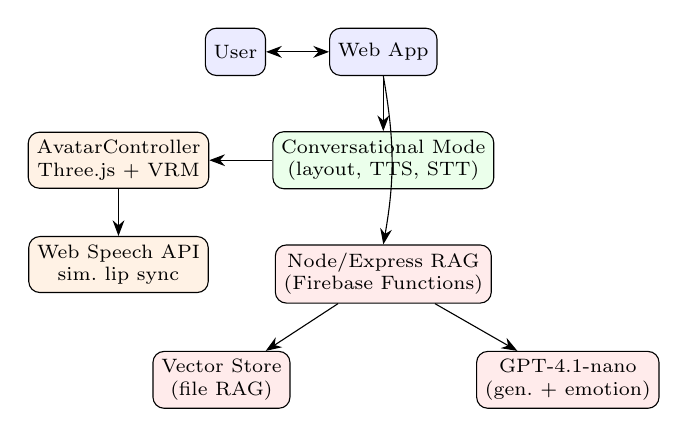
\begin{tikzpicture}[
  font=\scriptsize,
  box/.style={draw, rounded corners, align=center, inner sep=3pt, minimum height=6mm},
  >={Stealth[length=2mm]}]
\node[box, fill=blue!8] (user) {User};
\node[box, fill=blue!8, right=8mm of user] (app) {Web App};
\node[box, fill=green!8, below=7mm of app] (toggle) {Conversational Mode\\(layout, TTS, STT)};
\node[box, fill=orange!10, left=8mm of toggle] (avatar) {AvatarController\\Three.js + VRM};
\node[box, fill=orange!10, below=6mm of avatar] (tts) {Web Speech API\\sim.\ lip~sync};
\node[box, fill=red!8, below=7mm of toggle] (back) {Node/Express RAG\\(Firebase Functions)};
\node[box, fill=red!8, below left=6mm and -2mm of back] (vec) {Vector Store\\(file RAG)};
\node[box, fill=red!8, below right=6mm and -2mm of back] (llm) {GPT-4.1-nano\\(gen.\ + emotion)};
\draw[<->] (user) -- (app);
\draw[->] (app) -- (toggle);
\draw[->] (toggle) -- (avatar);
\draw[->] (avatar) -- (tts);
\draw[->] (app.south) to[bend left=10] (back.north);
\draw[->] (back) -- (vec);
\draw[->] (back) -- (llm);
\end{tikzpicture}
\caption{Ariel architecture. The RAG/LLM back end is shared by both conditions;
the toggle enables or disables embodiment, voice and the avatar.}
\label{fig:arch}
\end{figure}


% =====================================================================
\section{Methodology}
\label{sec:method}

\textbf{Design.}
We ran a \emph{between-subjects expert pilot} with two conditions: A~(CVA:
3D~avatar~+~synthesized~voice~+~STT~+~animations) and B~(text baseline: same
platform with text chat only, no body or voice). An expert pilot was chosen
because evaluation with real end users would require approval from the
University of Costa Rica Scientific Ethics Committee, beyond the course
time frame; experts in HCI or document systems provide structured evaluative
feedback to refine the protocol. The between-subjects design avoids learning
effects and direct-comparison bias.

\textbf{Participants.}
Eight experts with academic or professional experience in HCI, information
retrieval, conversational agents or document management, randomly assigned to
condition ($n=4$ per condition). One additional textual participant (TXT-01) was
excluded for not completing all instruments, preserving a balanced $N=8$.
No personally identifiable data are reported.

\textbf{Test file.}
The file comprises three public, formal regulations of the University of Costa
Rica (Student/Assistant Hours; Student Academic Regime; University Community
Work, TCU), selected because their normative nature is representative of
the platform's files, their detail is unfamiliar to most participants (avoiding
prior-knowledge bias), and they contain specific, verifiable data enabling
objective retention questions.

\textbf{Tasks and instruments.}
Each participant performed three tasks: T1, a verification query
(factual answer, post-task TiA, RQ1); T2, a cross-regulation synthesis query
integrating two regulations (post-task Godspeed, RQ2); and T3, three
point-data queries with objectively verifiable answers (triple the
student-hour wage; minimum passing grade $7.0$; minimum $8$ students per TCU
project), feeding the retention questionnaire, with SUS administered post-session
(RQ3). Instruments: TiA \cite{jian2000} (12 items, 7-point), Godspeed
\cite{bartneck2009} (5-point semantic differential), SUS \cite{brooke1996}
(10 items, normalized 0--100) and an ad-hoc 3-item retention questionnaire,
plus evaluator notes and a 5-question semi-structured closing interview
(Nielsen-style structured observation \cite{nielsen1994}).

\textbf{Procedure and analysis.}
Sessions (45--55\,min) followed: consent, brief practice, T1--T3 with
between-task instruments, SUS, and closing interview. Given the small sample,
analysis is descriptive (means, standard deviations, trend comparison),
complemented by qualitative interview coding. This pilot does not seek
statistical significance but informs protocol refinement for a future study with
real users.


% =====================================================================
\section{Results}
\label{sec:results}

Table~\ref{tab:quant} summarizes the quantitative results by condition; the
Godspeed subscales appear in Table~\ref{tab:godspeed}.

\textbf{Perceived trust (TiA, RQ1).}
The CVA condition showed higher perceived trust on the positive trust items
(mean $4.83$ vs.\ $3.58$ on a 7-point scale), with comparably low distrust
($2.15$ vs.\ $1.85$). The trust response was, however, heterogeneous: one CVA
expert rated trust low ($2/7$), reporting that the very speed of the answers
raised suspicion. Textual participants anchored their trust on directly seeing
the cited article in the PDF (``what made me trust it was seeing the article to
verify'').

\textbf{Interaction naturalness (Godspeed, RQ2).}
Counter to the embodiment hypothesis, the CVA was rated \emph{lower} than the
text interface on anthropomorphism ($1.60$ vs.\ $2.50$), animacy
($2.00$ vs.\ $3.04$), likeability ($3.15$ vs.\ $3.85$) and perceived safety
($3.25$ vs.\ $4.00$). Perceived intelligence was essentially equal
($3.80$ vs.\ $3.90$). Every CVA participant spontaneously flagged the synthetic
voice and rigid movement as artificial (``it's not natural\dots evaluating the
voice, it's not natural, the mouth doesn't move properly''; ``more realistic,
less of a manga cartoon'').

\textbf{Usability and retention (SUS, RQ3).}
SUS was equivalent and above the $68$ acceptability threshold in both conditions
($73.8$ vs.\ $72.5$). Retention was likewise equivalent and high
($2.25$ vs.\ $2.50$ out of $3$). Embodiment neither helped nor hurt usability or
effective information transfer; both interfaces were described as fast, easy and
intuitive.

\begin{table}[t]
\caption{Quantitative results by condition (mean\,$\pm$\,SD, $N=8$).}
\label{tab:quant}
\centering
\renewcommand{\arraystretch}{1.2}
\begin{tabular}{@{}lccc@{}}
\toprule
\textbf{Metric} & \textbf{A: CVA} ($n{=}4$) & \textbf{B: Text} ($n{=}4$) & \textbf{RQ} \\
\midrule
TiA trust (1--7)      & $4.83 \pm 2.01$ & $3.58 \pm 2.15$ & RQ1 \\
TiA distrust (1--7)   & $2.15 \pm 0.90$ & $1.85 \pm 0.38$ & RQ1 \\
SUS (0--100)          & $73.8 \pm 6.0$  & $72.5 \pm 14.9$ & RQ3 \\
Retention (0--3)      & $2.25 \pm 0.96$ & $2.50 \pm 1.00$ & RQ3 \\
\bottomrule
\end{tabular}
\end{table}

\begin{table}[t]
\caption{Godspeed subscales (1--5 semantic differential).}
\label{tab:godspeed}
\centering
\renewcommand{\arraystretch}{1.2}
\begin{tabular}{@{}lcc@{}}
\toprule
\textbf{Subscale} & \textbf{A: CVA} & \textbf{B: Text} \\
\midrule
Anthropomorphism        & $1.60 \pm 0.85$ & $2.50 \pm 0.53$ \\
Animacy                 & $2.00 \pm 0.65$ & $3.04 \pm 0.75$ \\
Likeability             & $3.15 \pm 0.57$ & $3.85 \pm 0.84$ \\
Perceived intelligence  & $3.80 \pm 0.75$ & $3.90 \pm 0.26$ \\
Perceived safety        & $3.25 \pm 0.50$ & $4.00 \pm 0.00$ \\
\bottomrule
\end{tabular}
\end{table}


% =====================================================================
\section{Discussion}
\label{sec:discussion}

\textbf{RQ1: embodiment raised perceived trust.}
On average the CVA produced higher trust (TiA $4.83$ vs.\ $3.58$) with similarly
low distrust, consistent with literature reporting that visual presence and
voice increase perceived trust and social presence \cite{wang2019,chang2022,
schmitt2022}. The effect was not uniform: the dominant trust cue in \emph{both}
conditions was the verifiable source---textual users trusted because they could
see the cited article, echoing the RAG principle that grounding in a verifiable
memory underpins reliability \cite{fan2024,roy2024}. Embodiment therefore acts
as a trust amplifier layered on top of source visibility, not as a substitute
for it. A practical implication is that a CVA should make its sources explicit
and visible, since immediacy alone can paradoxically breed suspicion (the
``too-fast'' answers reported by one expert).

\textbf{RQ2: embodiment, as implemented, lowered perceived naturalness.}
The most salient---and counterintuitive---finding is that the embodied agent
scored \emph{below} the plain text interface on anthropomorphism, animacy and
likeability. This is consistent with the Uncanny Valley \cite{mori2012}: a body
with low-fidelity multimodal output (browser-synthesized voice, simulated
lip~sync decoupled from real audio, procedural-but-rigid motion, a stylized
manga avatar) introduces artificiality cues that a familiar, frictionless text
chat simply does not have. The qualitative data converge unanimously on voice
and movement as the culprits, while perceived intelligence---driven by the
shared RAG/LLM back end---remained equal across conditions. The lesson aligns
with work on multimodal feedback and lip~sync \cite{chang2022,elfleet2024,
alalyani2023}: the presence of a body is not sufficient; its perceived
naturalness is gated by the fidelity and synchronization of voice and motion.

\textbf{RQ3: embodiment was usability- and retention-neutral.}
SUS was acceptable and statistically indistinguishable between conditions, and
retention was high in both, indicating that the identical RAG core delivered the
factual content equally well regardless of presentation. Embodiment did not
impose a usability cost---an encouraging result---but also did not improve
comprehension, in contrast with high-impact multimodal results elsewhere
\cite{yang2025health}, plausibly because our task is short, factual and
text-anchored (the PDF is always visible).

\textbf{Synthesis.}
Embodiment improved trust, degraded perceived naturalness, and left usability
and retention unchanged. The dissociation indicates that the bottleneck is
\emph{multimodal fidelity}, not embodiment per se: the same body that lent
authority hurt naturalness because its voice and motion were synthetic. This
reframes the design goal from ``add an avatar'' to ``raise voice and animation
fidelity to the level where embodiment's trust benefit is not offset by an
artificiality penalty.''

\textbf{Limitations.}
The pilot is small ($N=8$) and descriptive, without statistical power; experts
are not the end-user population; the between-subjects design precludes
within-subject comparison; the synthetic-voice/simulated-lip~sync prototype
likely represents a lower bound on achievable CVA naturalness; and the
single-session, short-task setting limits ecological validity. The retention
and TiA SDs are wide, so trends should be read as hypotheses for a larger study.


% =====================================================================
\section{Conclusions and Future Work}
\label{sec:conclusion}

We presented Ariel, a web-native corporeal virtual agent (Three.js + VRM) over a
RAG back end, and a controlled between-subjects pilot isolating embodiment in a
document-consultation task. The evidence shows a clear dissociation: embodiment
\emph{increased perceived trust} (TiA $4.83$ vs.\ $3.58$) but \emph{decreased
perceived naturalness} (anthropomorphism $1.60$ vs.\ $2.50$), while leaving
usability (SUS $73.8$ vs.\ $72.5$) and retention ($2.25$ vs.\ $2.50/3$)
unchanged. Qualitative data attribute the naturalness penalty to low-fidelity
voice and motion rather than to embodiment itself, indicating that multimodal
fidelity---not the mere presence of a body---is the decisive design variable.
Future work should replace browser TTS with high-fidelity neural voices and
audio-driven lip~sync, test more realistic avatars, and always surface verifiable
sources to consolidate the trust benefit.

\textbf{Publication projection.} At present there is \emph{no} plan to submit
this study to the Scientific Ethics Committee or to pursue formal data collection
for academic publication; the work is conducted as a course research exercise.
Should the prototype's multimodal fidelity be improved, a larger study with real
users would be the natural next step toward publication.


% =====================================================================
\begin{thebibliography}{99}
\bibitem{fan2024} W. Fan \emph{et al.}, ``A Survey on RAG Meeting LLMs: Towards Retrieval-Augmented Large Language Models,'' in \emph{Proc. 30th ACM SIGKDD}, 2024. doi:10.1145/3637528.3671470.
\bibitem{zerhoudi2024} S. Zerhoudi and M. Granitzer, ``PersonaRAG: Enhancing Retrieval-Augmented Generation Systems with User-Centric Agents,'' arXiv:2407.09394, 2024. doi:10.48550/arXiv.2407.09394.
\bibitem{more2025} A. More, ``Interaction via Large Language Models: Advancements in Retrieval-Augmented Intelligent Interfaces,'' \emph{IJRASET}, vol.\ 13, no.\ 5, 2025. doi:10.22214/ijraset.2025.70382.
\bibitem{alalyani2023} N. Alalyani and N. Krishnaswamy, ``A Methodology for Evaluating Multimodal Referring Expression Generation for Embodied Virtual Agents,'' in \emph{Companion Proc. ICMI}, 2023. doi:10.1145/3610661.3616548.
\bibitem{schmitt2022} A. Schmitt, T. Wambsganss, and J. M. Leimeister, ``Conversational Agents for Information Retrieval in the Education Domain: A User-Centered Design Investigation,'' \emph{Proc. ACM Hum.-Comput. Interact.}, vol.\ 6, no.\ CSCW2, 2022. doi:10.1145/3555587.
\bibitem{egelhofer2025} D. Egelhofer \emph{et al.}, ``Effects of Verbal Interruption in Conversations with an Intelligent Virtual Agent in Virtual Reality,'' in \emph{Proc. ACM SUI}, 2025. doi:10.1145/3694907.3765918.
\bibitem{wang2019} I. Wang, J. Smith, and J. Ruiz, ``Exploring Virtual Agents for Augmented Reality,'' in \emph{Proc. CHI}, 2019. doi:10.1145/3290605.3300511.
\bibitem{chang2022} Z. Chang \emph{et al.}, ``The Impact of Virtual Agents' Multimodal Communication on Brain Activity and Cognitive Load in Virtual Reality,'' \emph{Front. Virtual Real.}, vol.\ 3, 2022. doi:10.3389/frvir.2022.995090.
\bibitem{jolibois2025} S. C. Jolibois, A. Ito, and T. Nose, ``The Development of an Emotional Embodied Conversational Agent and the Evaluation of the Effect of Response Delay on User Impression,'' \emph{Appl. Sci.}, vol.\ 15, no.\ 8, 4256, 2025. doi:10.3390/app15084256.
\bibitem{yang2025ar} H.-K. Yang \emph{et al.}, ``An Embodied AR Navigation Agent: Integrating BIM with Retrieval-Augmented Generation for Language Guidance,'' in \emph{Proc. IEEE ISMAR}, 2025. doi:10.1109/ISMAR67309.2025.00150.
\bibitem{yang2025health} H. Yang, Q. Tian, and X. Gu, ``Toward Industry 5.0: Evaluating Multimodal Virtual Human Interaction for Smart Healthcare in Simulated VR Environments,'' \emph{Internet Technol. Lett.}, vol.\ 9, e70190, 2026. doi:10.1002/itl2.70190.
\bibitem{elfleet2024} M. Elfleet and M. Chollet, ``Investigating the Impact of Multimodal Feedback on User-Perceived Latency and Immersion with LLM-Powered ECAs in VR,'' in \emph{Proc. ACM IVA}, 2024. doi:10.1145/3652988.3673965.
\bibitem{zhu2024} Y. Zhu \emph{et al.}, ``Retrieval-Augmented Embodied Agents,'' in \emph{Proc. IEEE/CVF CVPR}, 2024. doi:10.1109/CVPR52733.2024.01703.
\bibitem{roy2024} S. Roy, M. Goswami, and S. Mohanty, ``Conversational Text Extraction with Large Language Models Using Retrieval-Augmented Systems,'' in \emph{Proc. IEEE CINE}, 2024. doi:10.1109/CINE63708.2024.10881808.
\bibitem{haque2025} I. C. R. Haque, ``Implementation of RAG and LLM for a Document and Tabular-Based Chatbot System,'' \emph{JOETEX}, vol.\ 3, no.\ 1, 2025. doi:10.52465/joetex.v3i1.588.
\bibitem{ahn2022} Y. Ahn, S.-G. Lee, J. Shim, and J. Park, ``Retrieval-Augmented Response Generation for Knowledge-Grounded Conversation in the Wild,'' \emph{IEEE Access}, vol.\ 10, 2022. doi:10.1109/ACCESS.2022.3228964.
\bibitem{liang2025} Y. Liang, Z. Wu, F. Zhang, D. Song, and H. Huang, ``How Users Interact with Generative Information Retrieval Systems: A Study of User Behavior and Search Experience,'' in \emph{Proc. 48th ACM SIGIR}, 2025. doi:10.1145/3726302.3729998.
\bibitem{shimadzu2025} H. Shimadzu, T. Utsuro, and D. Kitayama, ``Retrieval-Augmented Simulacra: Generative Agents for Up-to-Date and Knowledge-Adaptive Simulations,'' in \emph{Proc. IEEE GCCE}, 2025. doi:10.1109/GCCE65946.2025.11275306.
\bibitem{koleva2024} K. Koleva, M. Vergari, T. Koji\'{c}, S. M\"{o}ller, and J.-N. Voigt-Antons, ``Influence of Personality and Communication Behavior of a Conversational Agent on User Experience and Social Presence in Augmented Reality,'' in \emph{Proc. IEEE VRW}, 2024. doi:10.1109/VRW62533.2024.00261.
\bibitem{calvo2025} R. Calvo, H. Wang, A. Barquero, X. Zhang, R. Venkatakrishnan, and J. Ruiz, ``Exploring Interactions with Companion Virtual Agents,'' in \emph{Proc. 13th Int. Conf. Human-Agent Interaction (HAI)}, 2025. doi:10.1145/3765766.3765791.
\bibitem{jian2000} J.-Y. Jian, A. M. Bisantz, and C. G. Drury, ``Foundations for an Empirically Determined Scale of Trust in Automated Systems,'' \emph{Int. J. Cognitive Ergonomics}, vol.\ 4, no.\ 1, pp.\ 53--71, 2000. doi:10.1207/S15327566IJCE0401\_04.
\bibitem{bartneck2009} C. Bartneck, D. Kuli\'{c}, E. Croft, and S. Zoghbi, ``Measurement Instruments for the Anthropomorphism, Animacy, Likeability, Perceived Intelligence, and Perceived Safety of Robots,'' \emph{Int. J. Social Robotics}, vol.\ 1, no.\ 1, pp.\ 71--81, 2009. doi:10.1007/s12369-008-0001-3.
\bibitem{brooke1996} J. Brooke, ``SUS: A Quick and Dirty Usability Scale,'' in \emph{Usability Evaluation in Industry}, pp.\ 189--194, 1996.
\bibitem{mori2012} M. Mori, K. F. MacDorman, and N. Kageki, ``The Uncanny Valley,'' \emph{IEEE Robot. Autom. Mag.}, vol.\ 19, no.\ 2, pp.\ 98--100, 2012. doi:10.1109/MRA.2012.2192811.
\bibitem{nielsen1994} J. Nielsen, \emph{Usability Engineering}. San Francisco, CA: Morgan Kaufmann, 1994.
\end{thebibliography}

\end{document}
